\documentclass[11pt]{article}
\usepackage[margin=1.15in]{geometry}
\usepackage{amsmath,amssymb,amsthm}
\usepackage{booktabs}
\usepackage{array}
\usepackage{microtype}
\usepackage{tikz}
\usetikzlibrary{arrows.meta,positioning,calc}
\usepackage[hidelinks]{hyperref}
\usepackage{setspace}
\setstretch{1.08}

\newtheorem{proposition}{Proposition}[section]
\newtheorem{theorem}[proposition]{Theorem}
\newtheorem{corollary}[proposition]{Corollary}
\newtheorem{lemma}[proposition]{Lemma}
\theoremstyle{definition}
\newtheorem{definition}[proposition]{Definition}
\newtheorem{example}[proposition]{Example}
\theoremstyle{remark}
\newtheorem{remark}[proposition]{Remark}

\newcommand{\negl}{\mathsf{negl}}
\newcommand{\R}{\mathbb{R}}
\newcommand{\Hmin}{H_{\infty}}
\DeclareMathOperator{\rank}{rank}
\DeclareMathOperator{\Pro}{Pr}

\title{Distributed Material Archives:\\
Multidimensional Optical Encoding, Embedded Manufacture,\\
and the Physical Replication of Public Knowledge}
\author{Flyxion\\Independent Researcher}
\date{October 2026}

\begin{document}
\maketitle

\begin{abstract}
\noindent This essay specifies a research program in which digital archives are written into optically distinguishable structures during the fabrication of ordinary manufactured objects, so that bricks, tiles, tabletops, printed components, and textiles could carry replicated public knowledge as a routine by-product of manufacture. The central difficulty is a confusion between three quantities that popular accounts of multidimensional storage tend to merge: the number of possible inscriptions, the amount of information that one inscription can reliably carry, and the number of independently recoverable archives that can share one physical region. The first grows exponentially with the number of adjustable fabrication parameters, the second grows only linearly in the same parameters, and the third is bounded by the second. The essay develops these distinctions as theorems with complete proofs, derives capacity bounds under bounded and Gaussian noise, specifies a reader architecture at the level of its analogue front end, digital controller, and error-correcting back end, and treats the steganographic and cryptographic aspects of an archive that is meant to be both unobtrusive and publicly recoverable. Numerical studies are carried out for twelve, one hundred forty-four, and thirteen thousand adjustable parameters, and the resulting tables are conditional calculations that depend on explicit physical assumptions. Material capacities, endurance, and manufacturing yield remain experimental questions, and the final sections lay out the experimental sequence, the controls, and the conditions under which the program would fail.
\end{abstract}

\tableofcontents
\newpage

\section{From Dedicated Storage Devices to Archival Manufacture}\label{sec:intro}

Digital knowledge currently survives through a chain of dependencies that are rarely examined together: functioning organizations that host it, networks that deliver it, accounts that authorize access to it, electricity that powers the machines that hold it, and specialized storage equipment whose formats are understood by a small number of manufacturers. Each link is individually reliable, and the chain as a whole has proved durable for a few decades, but it is a chain, and a failure at any link removes access for everyone downstream. The proposal examined here concerns a different mode of survival. Selected public archives would travel not only through dedicated storage devices but also through manufacturing and construction, so that reference collections might be embodied in tiles, technical manuals embedded in replacement parts, and dated encyclopedic snapshots distributed with household objects. The archive would then persist for the same reason that a pattern in a brick persists, namely that the object is useful for other reasons and is therefore made, shipped, installed, and kept.

The motivating object is an ordinary brick carrying two inscriptions. The first is an obvious and sparse introductory inscription that states what the object contains and how to read it. The second is a dense optical archive written into a face or into the volume of the unit during manufacture. This single example poses the entire problem at once. The archive must survive manufacture, which subjects it to heat, pressure, shrinkage, and handling. It must remain discoverable by someone who does not know it is there, which requires that the introductory layer be recognizable. It must permit alignment and calibration of a reader to the particular specimen, since no two bricks are identical. It must identify its own format. And it must yield verified files through a reader that an independent party can reconstruct from published specifications, because an archive that can be read only with a proprietary scanner, a cloud account, or an undocumented decoding model has replaced one dependency with another.

The value of such a scheme has two distinct sources that the essay keeps apart throughout. The first is density, meaning the number of recoverable bits per unit area or volume of material. The second is distribution, meaning the number of independent physical copies and the diversity of the objects and places that hold them. A modest archive replicated across millions of ordinary objects could be socially consequential even if its density never exceeded that of specialized archival media, because the consequence derives from the cost of replication and the dispersal of copies rather than from the packing of bits. Conversely, an extraordinarily dense medium confined to a few vaults provides the vulnerability of centralized storage regardless of how much each vault holds. Density determines how large an archive an object of a given size can carry, and distribution determines how likely it is that some copy survives, and the program must establish both.

The technical argument is organized as follows. Section~\ref{sec:foundations} situates the proposal among existing work on laser-written glass, volume holography, and multiplexed optical encoding, and identifies what a new contribution would have to be. Section~\ref{sec:defs} fixes the vocabulary that separates addresses from payloads and fabrication controls from observable states. Section~\ref{sec:model} introduces the write--store--read model on which every later claim rests. Sections~\ref{sec:capacity} through~\ref{sec:fixed} develop the mathematical core: the combinatorial capacity of a product alphabet, geometric scaling to areas and volumes, the limiting role of observational equivalence, robust capacity as a packing problem, overlapping storage, linear multiplexing with crosstalk, and fixed-resource scaling in a Gaussian channel. Sections~\ref{sec:substrates} through~\ref{sec:ecc} address substrates, reader circuits, calibration and self-description, and error correction. Section~\ref{sec:stego} treats concealment and confidentiality, which for an archive intended to be publicly recoverable are in tension with the principal design goal and therefore require careful accounting. Sections~\ref{sec:experiments} through~\ref{sec:distribution} specify the experimental sequence, the controls, and the system-level analysis of replication. Section~\ref{sec:popular} returns to the broader vision in a less formal register, and Section~\ref{sec:program} lays out the resulting publication program. Appendices collect worked budgets, a container format, and the notation.

\section{Existing Foundations and the Proposed Contribution}\label{sec:foundations}

The proposal stands on substantial prior engineering, and the purpose of this section is to identify that foundation precisely enough that the contribution of the present program can be stated without overclaiming. Laser writing in glass is the nearest precedent. Early demonstrations of five-dimensional recording in glass combined three spatial coordinates with two optical properties of laser-induced nanostructures, namely the orientation and the strength of the retardance that the structure induces in transmitted light, and showed that polarization-controlled material modifications could carry digital information \cite{zhang2013}. Subsequent work demonstrated multilayer recording with error-free recovery over many layers in silica \cite{wang2022}. The most developed recent result, reported by the Project Silica team, integrates inscription, optical readout, decoding, error correction, and retention testing, and reports usable capacities of several terabytes in a single glass specimen of standard plate dimensions \cite{silica2026}. The accompanying systems literature considers how such a medium becomes part of an archival architecture rather than remaining a laboratory demonstration \cite{anderson2023}. These results establish that volumetric optical archiving in glass is a real engineering discipline with measured capacities. They do not establish that comparable performance transfers to stone, ceramic, cloth, or the heterogeneous materials of the built environment, and the present program treats that transfer as an open experimental question.

A second body of work concerns holographic data storage, in which data are encoded as interference patterns and multiple pages share a volume through angular, wavelength, or phase multiplexing. The foundational reference collects the theory of recording media, multiplexing, optical architectures, and system optimization \cite{coufal2000}, and a recent survey examines the density, energy efficiency, and switching difficulties that have repeatedly prevented holographic storage from displacing competing technologies \cite{cheriere2025}. That survey is an essential counterweight to capacity arguments based solely on nominal degrees of freedom, because it records the dynamic-range and interference limits that appear when many holograms share a material.

A third body of work concerns fabricated metasurfaces, in which structure at or below the wavelength scale controls the phase, amplitude, and polarization of reflected or transmitted light. Metasurface holography has demonstrated orbital-angular-momentum multiplexing in momentum space with complex-amplitude control \cite{ren2020}, and structural multiplexing with diffractive neural networks in three-dimensionally printed elements \cite{fan2024}. Those demonstrations concern reconstructed images, and image fidelity should not be equated with verified digital-file capacity, since the error criterion for an archive is exact recovery of every bit after error correction rather than perceptual similarity.

Optical research already investigates multiplexing through wavelength, polarization, incident angle, and orbital angular momentum, so the general observation that light supplies many usable degrees of freedom is not a contribution. The contribution of the present program, if it has one, must be located in one of four places: a specific encoding architecture whose capacity is established under an explicit error criterion; a fabrication method that writes the encoding during ordinary manufacture rather than in a dedicated inscription step; a reader that can be reconstructed independently from published specifications; or an archival system that makes replication across everyday objects operationally meaningful. The essay develops all four at the level of specification and bounds, and the experimental sections state which claims each experiment would support or refute.

The mathematical apparatus is deliberately elementary, since the central difficulty lies in stating the counting problem correctly rather than in advanced technique. Counting principles, functions and relations, equivalence classes, and the pigeonhole principle, as presented in standard discrete mathematics texts \cite{epp,kolman}, suffice for the first half of the development. Shannon's framework for reliable communication through noisy channels \cite{shannon1948,cover2006} supplies the second half. Digital control and circuit analysis are treated using the standard treatments of logic design \cite{mano} and linear circuits \cite{boylestad}, supplemented in Section~\ref{sec:reader} by specialized references that a final bibliography would add for photodetection and optical design.

\section{Definitions: What Is Being Counted}\label{sec:defs}

Most errors in popular discussions of multidimensional storage arise from counting the wrong thing, and the definitions below are chosen to make the intended count explicit. A \emph{manufacturing control} is an adjustable input to the fabrication process, such as pulse duration, pulse energy, inscription orientation, feature depth, spatial frequency, layer position, or composition. A \emph{material state} is the physical configuration that results from fabrication, which depends on the controls and also on the substrate and on process variation. A \emph{readout observable} is a measurable response of a material state under a specified reader configuration, such as transmitted intensity, retardance, scattering angle, or phase. A \emph{recoverable symbol} is a member of a codebook whose elements are distinguishable under stated operating conditions with a stated error probability. These four notions form a chain from what the manufacturer adjusts to what the reader can decide, and a count taken at the first link says nothing about a count taken at the last.

Three distinctions follow, each of which prevents a specific accounting error. The first is between controls and states: several different settings of the controls can produce the same material state, as when two pulse widths leave the same mark, so the number of control settings overstates the number of states. The second is between states and observations: different material states can produce indistinguishable observations, so the number of states overstates the number of recoverable symbols. The third is between an address and a payload: an enormous space of possible inscriptions is an address space, and it becomes a storage capacity only to the extent that each address can be written and read reliably and carries information that the reader did not already possess. A physical storage \emph{site} is a region that is written and read as a unit, and it must be distinguished from an optical \emph{mode}, which is one of several independently addressable components of the response of a single site. An overlapping archive, in which several collections share a region, must in turn be distinguished from an alternative interpretation of one archive, in which the same observations are decoded in different ways to yield different files, since only the former adds payload.

\begin{definition}[Capacity of a configuration space]\label{def:capacity}
Let $\mathcal U$ be a finite set of fabrication settings, $\mathcal Y$ the set of readout observations, and $\omega:\mathcal U\to\mathcal Y$ the nominal readout map. A \emph{zero-error codebook} is a subset $\mathcal K\subseteq\mathcal U$ on which $\omega$ is injective, and the \emph{zero-error capacity} of one site is $\lfloor\log_2 |\omega(\mathcal U)|\rfloor$ bits, which equals the logarithm of the number of distinct observations that the reader can produce.
\end{definition}

The definition has a consequence that will be used repeatedly: capacity is a property of the image of the readout map and not of its domain. The number of fabrication settings, which is the quantity that grows without limit as parameters are added, enters the capacity only through the number of distinct observations those settings produce.

\section{The Complete Write--Store--Read Model}\label{sec:model}

Every capacity claim in the essay refers to the following chain of operations, which makes the roles of substrate variation, ageing, and reader configuration explicit:
\[
X\xrightarrow{\;E\;}U\xrightarrow{\;F_s\;}Z_0\xrightarrow{\;D_t\;}Z_t\xrightarrow{\;R_v\;}Y\xrightarrow{\;G\;}\widehat X .
\]
Here $X$ is the source message, $E$ the encoder, which includes compression, error-correcting coding, and the mapping from coded symbols to fabrication settings, $U$ the resulting fabrication instructions, $F_s$ the substrate-dependent fabrication process indexed by a vector $s$ of substrate and process conditions, $Z_0$ the as-fabricated material state, $D_t$ the degradation process over time $t$, $Z_t$ the aged state, $R_v$ the reader operating under configuration $v$, $Y$ the raw observation, $G$ the decoder, and $\widehat X$ the recovered message. The maps $F_s$, $D_t$, and $R_v$ are random in general, and the model should be read as a composition of channels rather than of deterministic functions.

The decomposition matters because failures belong to different links and have different remedies. A decoder may work on an ideal simulation and fail after printing shrinkage, which is a failure of $F_s$. A physical inscription may remain stable for centuries while its reader becomes unavailable, which is a failure of $R_v$ and of the documentation that would permit its reconstruction. An inscription that is fully readable on the day of manufacture may be unreadable after abrasion or weathering, which is a failure of $D_t$. A program that measured only the first link would overstate the usefulness of an archive, and all three kinds of failure belong within the research program.

The primary performance condition is
\begin{equation}\label{eq:perr}
\Pro\bigl(\widehat X\neq X\bigr)\le\varepsilon,
\end{equation}
evaluated under a specified distribution of manufacturing conditions $s$, environmental exposures $t$, and reader tolerances $v$. Every capacity claim in the essay is accompanied by a statement of $\varepsilon$ and of that distribution, because a capacity without an error criterion is not a well-defined quantity. For an archive of verified files the natural criterion is exact recovery of each block after error correction, with a small $\varepsilon$ per block and an explicit policy for blocks that cannot be recovered.

\section{The Combinatorial Capacity Theorem}\label{sec:capacity}

The first proposition establishes precisely the exponential growth that motivates the program, together with the less celebrated fact that payload grows only linearly in the number of properties.

\begin{proposition}[Distinguishable product states]\label{prop:product}
Suppose a storage element supports $d$ independently selectable and jointly distinguishable properties, and that property $i$ has $L_i\ge 2$ usable levels. The complete product alphabet then contains
\[
M=\prod_{i=1}^{d}L_i
\]
states, and the maximum fixed-length binary payload of one element is
\[
b=\bigl\lfloor\log_2 M\bigr\rfloor=\Bigl\lfloor\sum_{i=1}^{d}\log_2 L_i\Bigr\rfloor .
\]
\end{proposition}

\begin{proof}
The set of joint states is the Cartesian product of the sets of levels, whose cardinality is the product of the cardinalities, which gives $M$. An injective encoding of all $b$-bit messages into the $M$ states exists if and only if $2^b\le M$, so the largest admissible $b$ is $\lfloor\log_2 M\rfloor$. The second form follows because the logarithm of a product is the sum of the logarithms.
\end{proof}

\begin{corollary}[Linear growth of payload]\label{cor:linear}
If every property has the same number of levels $L$, then $M=L^{d}$ and $b=\lfloor d\log_2 L\rfloor$. Adding one independent property multiplies the number of states by $L$ and adds exactly $\log_2 L$ bits to the payload.
\end{corollary}

The corollary is the most important sentence in the quantitative argument. The number of possible inscriptions, which is the number of joint states, grows exponentially in $d$ and quickly exceeds any physical count, while the information that an element carries, which is the logarithm of that number, grows only linearly. An immense repertoire of patterns is therefore compatible with a modest payload, and the repertoire by itself does not demonstrate storage. The joint distinguishability assumption in Proposition~\ref{prop:product} is also an assumption to be demonstrated for each candidate set of properties, and the later sections of the essay explain how it fails.

With sixteen distinguishable levels per property, so that each property contributes four bits, the illustrative cases are those of Table~\ref{tab:states}. The state counts in the table were computed directly from $2^{4d}$.

\begin{table}[h]
\centering
\small
\begin{tabular}{@{}rrrr@{}}
\toprule
Independent properties $d$ & Joint states $16^{d}$ & Information per element & Bytes per element \\
\midrule
12 & $2^{48}\approx 2.81\times10^{14}$ & 48 bits & 6 \\
144 & $2^{576}\approx 2.47\times10^{173}$ & 576 bits & 72 \\
13{,}000 & $2^{52{,}000}\approx 3.63\times10^{15{,}653}$ & 52{,}000 bits & 6{,}500 \\
\bottomrule
\end{tabular}
\caption{Product-alphabet capacity with sixteen reliably distinguishable levels per property. State counts are exact exponents converted to scientific notation.}
\label{tab:states}
\end{table}

The last row supplies an astronomical repertoire of possible inscriptions, a number with more than fifteen thousand decimal digits, which exceeds by an enormous margin the commonly cited order of $10^{80}$ for the number of atoms in the observable universe, and the same row states honestly that the corresponding payload is 6.5 kilobytes per element, under exceptionally strong physical assumptions. The two halves of that sentence belong together in any statement of the result. The case for a research program does not require the first half alone, since 6.5 kilobytes at every site of a surface at modest pitch is already a very large capacity, as the next section computes, and the astronomical repertoire becomes relevant for a different purpose, namely that it makes exhaustive search over fabrication settings infeasible, which is a property of the address space and not of the stored information.

The proposition counts a single alphabet. Two refinements are needed for real designs. First, the levels need not be equal across properties, and a property that supports only two reliably distinguishable levels contributes one bit while one that supports sixty-four contributes six. Second, the floor in the formula applies once to the total and not to each term, so that a collection of properties with non-power-of-two level counts can still use mixed-radix coding to avoid wasting fractional bits. A property with three levels contributes $\log_2 3\approx 1.585$ bits to the total, and twenty such properties contribute 31.7 bits, so thirty-one bits can be stored across twenty ternary properties by representing the payload in a mixed-radix numeral system.

\section{Geometric Scaling from Elements to Objects}\label{sec:geometry}

The next step translates capacity per element into capacity per area and per volume. For a square surface array with element pitch $p$, usable area $A$, and payload $b$ bits per element,
\begin{equation}\label{eq:braw}
B_{\mathrm{raw}}=\Bigl\lfloor\frac{A}{p^{2}}\Bigr\rfloor\,b .
\end{equation}
For a layered volume with $n_\ell$ independently readable layers, the same expression is multiplied by $n_\ell$, and for a volume of side-by-side voxels with pitch $p$ in all three directions the number of sites is $\lfloor V/p^{3}\rfloor$.

A purely illustrative square metre with a pitch of $100\,\mu\mathrm{m}$ contains $10^{8}$ sites. Applying the assumptions of Table~\ref{tab:states}, the ideal raw capacities are given in Table~\ref{tab:area}, where decimal gigabytes are used and calibration, indexing, error correction, unusable sites, and other overhead are excluded.

\begin{table}[h]
\centering
\small
\begin{tabular}{@{}rrr@{}}
\toprule
Properties per site & Bits per site & Ideal raw capacity per square metre \\
\midrule
12 & 48 & 0.6\,GB \\
144 & 576 & 7.2\,GB \\
13{,}000 & 52{,}000 & 650\,GB \\
\bottomrule
\end{tabular}
\caption{Ideal raw capacity of a surface at $100\,\mu\mathrm{m}$ pitch ($10^{8}$ sites per square metre), sixteen levels per property.}
\label{tab:area}
\end{table}

The crucial qualification is that the parameter count $d$, the pitch $p$, and the reader resolution cannot in general be chosen independently. Supporting thirteen thousand observable properties at a site may require a much larger site, because each independent observable requires its own physical degree of freedom with enough response amplitude above the noise floor; it may require extensive sequential measurements, because the reader may have to illuminate and detect many times per site; or it may require a substantial optical volume per site, since the number of resolvable modes of a beam is bounded by the number of independent spatial and spectral degrees of freedom in its aperture. The experimental question is therefore whether the increase in information per site survives the increase in site size, measurement time, and cost. Writing $b(p)$ for the payload that can be supported at pitch $p$, the density is $b(p)/p^{2}$ per unit area, and a larger payload at a larger pitch beats a smaller payload at a smaller pitch only if $b$ grows faster than $p^{2}$. The program treats the function $b(p)$ as the central empirical object for each substrate.

\section{Observational Equivalence}\label{sec:equiv}

\begin{proposition}[Observational equivalence limits capacity]\label{prop:equiv}
In a deterministic readout model, call two writable configurations \emph{equivalent} if they produce identical observations under every permitted reader configuration. This is an equivalence relation on the set of configurations. A zero-error codebook contains at most one representative from each equivalence class, so the zero-error capacity is at most $\log_2 K$ bits, where $K$ is the number of equivalence classes.
\end{proposition}

\begin{proof}
Reflexivity, symmetry, and transitivity follow from the corresponding properties of equality of observations. Suppose a codebook contained two distinct equivalent configurations that were assigned to different messages. The decoder receives the same evidence for both and is a function of that evidence, so it returns the same output for both, and it is therefore wrong for at least one of the two messages. A zero-error codebook therefore has at most one configuration per class. The number of messages that can be assigned to distinct classes is at most $K$, which gives the stated bound.
\end{proof}

The proposition explains why increasing the number of fabrication controls does not necessarily increase storage capacity. It supplies a practical screening rule as well: a candidate parameter earns its place only if changing it changes recoverable observations under some permitted reader configuration, and a parameter that changes only the fabrication recipe is a distinction without a difference. The count of equivalence classes is also the object that Section~\ref{sec:experiments} proposes to estimate experimentally. In practice the equivalence is not exact, since noisy readout makes observations of nominally different configurations overlap with some probability, and the paper would replace exact equivalence by measured confusion probabilities and by distinguishability criteria.

For the noisy case the governing inequality is Fano's. If a message $X$ uniform over $M$ values is encoded, passed through any channel, and decoded from the observation $Y$, then
\[
\Pro(\widehat X\ne X)\;\ge\;1-\frac{I(X;Y)+1}{\log_2 M},
\]
where $I(X;Y)$ is the mutual information in bits \cite{cover2006}. The bound shows that reliable recovery of a message of $\log_2 M$ bits requires the channel to convey at least nearly that much mutual information, and it supplies the quantitative link between a measured confusion matrix and the payload that a site can be trusted with.

\section{Robust Capacity as a Packing Problem}\label{sec:packing}

\begin{proposition}[Bounded-noise decoding]\label{prop:bounded}
Suppose codeword $i$ produces a nominal observation $y_i\in\R^m$, and the readout error has norm at most $\delta$. If
\[
\min_{i\ne j}\|y_i-y_j\|>2\delta ,
\]
then nearest-neighbour decoding recovers every codeword correctly.
\end{proposition}

\begin{proof}
Let the true codeword be $i$ and the observation $y=y_i+e$ with $\|e\|\le\delta$. Then $\|y-y_i\|\le\delta$. For any $j\ne i$ the triangle inequality gives $\|y-y_j\|\ge\|y_i-y_j\|-\|y-y_i\|>2\delta-\delta=\delta$. The observation is therefore strictly closer to $y_i$ than to any competing nominal observation, and the nearest-neighbour rule returns $i$.
\end{proof}

The resulting research problem is a packing problem in observation space: how many sufficiently separated responses can the material and reader jointly support? The next result bounds the answer in the simplest nontrivial setting and shows that apparently continuous freedoms become a finite, experimentally meaningful codebook.

\begin{proposition}[Packing bounds under sup-norm noise]\label{prop:packing}
Let the nominal observations lie in the cube $[-R,R]^m$ and let the readout error satisfy $\|e\|_\infty\le\delta$ with $0<\delta\le R$. Any codebook that is decodable without error under this noise has at most $\bigl(1+R/\delta\bigr)^m$ codewords, and a codebook of $\lfloor R/\delta\rfloor^{m}$ codewords exists. Consequently the payload per site lies between $m\log_2\lfloor R/\delta\rfloor$ and $m\log_2(1+R/\delta)$ bits.
\end{proposition}

\begin{proof}
For the upper bound, decodability under every error of sup-norm at most $\delta$ requires that the cubes $y_i+[-\delta,\delta]^m$ be pairwise disjoint, since an observation in the intersection of two such cubes could have come from either codeword. Each such cube lies in $[-R-\delta,R+\delta]^m$, which has volume $(2(R+\delta))^m$, while each has volume $(2\delta)^m$. Disjointness gives $M(2\delta)^m\le(2(R+\delta))^m$, hence $M\le(1+R/\delta)^m$. For the lower bound, choose in each coordinate the points $-R+j(2\delta+\epsilon)$ for $j=0,1,\dots$ that lie in $[-R,R]$, with $\epsilon>0$ small. The number of such points is $\lfloor 2R/(2\delta+\epsilon)\rfloor+1$, which for sufficiently small $\epsilon$ is at least $\lfloor R/\delta\rfloor$. The product grid has pairwise sup-distance at least $2\delta+\epsilon>2\delta$ and is therefore decodable by Proposition~\ref{prop:bounded} in the sup norm, which is proved identically. Taking logarithms gives the payload range.
\end{proof}

The proposition is the sense in which a continuous parameter becomes a finite alphabet. A property measured over a range $R$ with noise $\delta$ supports between $\log_2\lfloor R/\delta\rfloor$ and $\log_2(1+R/\delta)$ bits, so the number of usable levels is the dynamic range divided by the noise width, and halving the noise buys one additional bit per property. The same calculation explains the dependence on the reader: improving measurement precision increases capacity only logarithmically, which is why capacity claims that depend on extremely fine resolution of a continuous variable should be treated with suspicion.

The program investigates three refinements. The first is anisotropic noise: the angle, depth, and intensity measurements of a site will have different ranges and different uncertainties, and the payload of a site with independent coordinates is $\sum_i\log_2\lfloor R_i/\delta_i\rfloor$ in the notation of the proposition applied coordinatewise. The second concerns systematic drift, which cannot be treated as independent random noise merely for convenience, since it is correlated across sites. One remedy is differential reading.

\begin{proposition}[Differential reading removes common offsets]\label{prop:diff}
Suppose every observation on a specimen is shifted by a common unknown offset $c\in\R^m$, so that $y=y_i+c+e$ with $\|e\|\le\delta$, and suppose a reference symbol with known nominal observation $y_0$ is observed as $y_{\mathrm{ref}}=y_0+c+e_0$ with $\|e_0\|\le\delta$. Then the difference $y-y_{\mathrm{ref}}=(y_i-y_0)+(e-e_0)$ is independent of $c$ and carries noise of norm at most $2\delta$. Nearest-neighbour decoding of the difference is correct whenever $\min_{i\ne j}\|y_i-y_j\|>4\delta$.
\end{proposition}

\begin{proof}
The algebraic identity eliminates $c$. Applying Proposition~\ref{prop:bounded} to the shifted nominal observations $y_i-y_0$ with noise bound $2\delta$ gives the separation condition $2(2\delta)=4\delta$.
\end{proof}

Differential reading therefore trades a doubling of the effective noise bound for immunity to any offset that is common to the symbol and its reference, at a cost of one bit per property if the codebook was previously separated by exactly $2\delta$ and the range is fixed. The third refinement is that offsets that vary across a specimen require references distributed densely enough that the offset is approximately constant between a symbol and its nearest reference, which is a requirement on the layout of calibration structures taken up in Section~\ref{sec:calibration}.

\section{Overlapping Storage and Independently Recoverable Channels}\label{sec:overlap}

This section formalizes the idea that several archives may occupy the same physical region and be read through different illumination conditions or decoding operations.

\begin{proposition}[Joint distinguishability requirement]\label{prop:overlap}
Let archive $j\in\{1,\dots,k\}$ have $M_j$ possible contents. If every combination of archive contents can be written into one region and every archive can be recovered without error from the available measurements, then the region supports at least $\prod_{j=1}^{k}M_j$ jointly distinguishable states, and the combined payload is
\[
B_{\mathrm{total}}=\sum_{j=1}^{k}\log_2 M_j .
\]
\end{proposition}

\begin{proof}
Consider the tuple of decoder outputs $(\widehat X_1,\dots,\widehat X_k)$. If two distinct tuples of archive contents produced identical complete observational evidence, the decoder would return the same tuple for both and would be wrong about at least one archive. Hence the map from the $\prod_j M_j$ tuples to total observational evidence is injective, so the number of distinguishable states of the region is at least the product, and its logarithm is the sum.
\end{proof}

Overlapping inscription can increase the utilization of a material region, but it does not remove the requirement that the reader obtain enough information to distinguish the joint contents. The proposition has a useful corollary for decoder side information. Suppose the decoder uses a dictionary, a trained model, or an external key $K$ that contains information about the archive contents. Then the recovered payload should be counted as $B_{\mathrm{total}}-H(K)$ in the worst case, since a decoder that already knows $H(K)$ bits of the answer has been given those bits outside the object. This closes a loophole by which a very large decoder could claim an arbitrarily large payload from a small physical inscription, and all experiments in Section~\ref{sec:experiments} disclose and account for decoder-resident information.

A convenient count for planning is the number of overlapping archives of a given size that a region can hold. A region of net capacity $B_{\mathrm{net}}$ bits holds at most $\lfloor B_{\mathrm{net}}/S\rfloor$ distinct archives of $S$ bits if all of them must be simultaneously recoverable and none is compressible against another. A square metre at the 144-property ideal of Table~\ref{tab:area} holds 7.2 gigabytes, which is seven hundred and twenty independent ten-megabyte archives, but it does not hold more, regardless of how many illumination conditions are available, unless those conditions yield additional jointly distinguishable observations.

\section{Linear Multiplexing, Rank, and Crosstalk}\label{sec:linear}

A tractable first model expresses the measured response as
\begin{equation}\label{eq:linear}
y=Ha+n,
\end{equation}
where $a\in\R^{d}$ contains the encoded mode amplitudes, $H\in\R^{m\times d}$ describes their mixing through the material and optics, and $n$ is measurement noise.

\begin{proposition}[Continuous identifiability]\label{prop:rank}
In the noiseless model $y=Ha$, arbitrary coefficient vectors $a\in\R^d$ are uniquely recoverable from $y$ if and only if $H$ has full column rank, that is, $\rank H=d$.
\end{proposition}

\begin{proof}
Suppose $\rank H<d$. Then the nullspace of $H$ contains a nonzero vector $v$, and $a$ and $a+v$ produce the same observation, so recovery fails for both. Conversely, if $\rank H=d$ then $H^{\top}H$ is invertible and $a=(H^{\top}H)^{-1}H^{\top}y$ is a left inverse.
\end{proof}

The result must be delimited carefully. A restricted finite codebook can remain distinguishable even when arbitrary continuous vectors are not identifiable. If $a_1\in\{0,1\}$ and $a_2\in\{0,2\}$, and the observation is the single number $y=a_1+a_2$, then $H=\begin{pmatrix}1&1\end{pmatrix}$ has rank one, yet the four codewords produce the four distinct observations $0,1,2,3$, and the payload of two bits is fully recoverable. Mixed-radix coding of this kind exploits the discreteness of the codebook to recover more than the rank of $H$ would suggest.

Full rank alone does not guarantee robust recovery, since very small singular values amplify noise. The next result quantifies the effect.

\begin{proposition}[Noise amplification]\label{prop:amp}
Let $H$ have full column rank with smallest singular value $\sigma_{\min}>0$, let the noise satisfy $\|n\|_2\le\delta$, and let a codebook $\mathcal A\subset\R^{d}$ satisfy $\|a-a'\|_2>2\delta/\sigma_{\min}$ for all distinct $a,a'\in\mathcal A$. Then nearest-neighbour decoding in observation space recovers every codeword correctly.
\end{proposition}

\begin{proof}
For distinct $a,a'\in\mathcal A$, the definition of the smallest singular value gives $\|H(a-a')\|_2\ge\sigma_{\min}\|a-a'\|_2>2\delta$. The nominal observations $Ha$ are therefore separated by more than $2\delta$, and Proposition~\ref{prop:bounded} applies in the Euclidean norm.
\end{proof}

A two-mode example shows the cost of crosstalk. Let $H=\begin{pmatrix}1&\kappa\\ \kappa&1\end{pmatrix}$ with $0\le\kappa<1$, whose singular values are $1+\kappa$ and $1-\kappa$. The sufficient condition of Proposition~\ref{prop:amp} requires coefficient spacing larger than $2\delta/(1-\kappa)$, which is $1/(1-\kappa)$ times the spacing needed without crosstalk, so over a fixed coefficient range the number of levels per mode shrinks by that factor and the payload per mode decreases by $\log_2\bigl(1/(1-\kappa)\bigr)$ bits. A crosstalk coefficient of $0.5$ costs one bit per mode, and one of $0.9$ costs more than three. The calculation is a sufficient-condition estimate and not a tight bound, but it shows how rapidly nominal parameter counts erode when modes mix.

The one hundred forty-four and thirteen thousand parameter studies therefore report singular-value spectra, confusion matrices, and decoding errors rather than nominal parameter counts. Holographic storage research has long identified material dynamic range and interference between multiplexed pages as the substantive constraints on multiplexing \cite{coufal2000,cheriere2025}, and the spectrum of $H$ is the compact way to express them: a spectrum that decays rapidly means that many of the nominal modes are effectively unobservable at the available signal-to-noise ratio.

\section{Fixed-Resource Scaling and the Cost of More Modes}\label{sec:fixed}

The article now asks what happens when total optical power, measurement time, detector area, and material volume are held fixed while the number of modes increases. An illustrative model uses $d$ parallel real Gaussian channels with equal noise variance $N$ and a total signal power $P$ divided equally among them, so that each carries $P/d$. The capacity of the combination, in bits per joint channel use, is
\begin{equation}\label{eq:gauss}
C(d)=\sum_{i=1}^{d}\tfrac12\log_2\Bigl(1+\frac{P_i}{N}\Bigr)=\frac d2\log_2\Bigl(1+\frac{P}{dN}\Bigr),
\end{equation}
under the normalization of real channels \cite{shannon1948,cover2006}.

\begin{proposition}[Saturation under a fixed power budget]\label{prop:gauss}
Let $x=P/N>0$. The function $C(d)$ of equation~\eqref{eq:gauss} is increasing in $d$ and bounded above by $x/(2\ln 2)$, and $C(d)\to x/(2\ln 2)$ as $d\to\infty$. Moreover, among all allocations $(P_1,\dots,P_d)$ with $\sum_iP_i=P$, the equal allocation maximizes the capacity.
\end{proposition}

\begin{proof}
Write $f(d)=d\ln(1+x/d)$, so that $C(d)=f(d)/(2\ln 2)$. Differentiating, $f'(d)=\ln(1+x/d)-\dfrac{x/d}{1+x/d}$, and since $\ln(1+u)\ge u/(1+u)$ for $u>0$, the derivative is nonnegative, so $f$ is increasing. The inequality $\ln(1+u)\le u$ gives $f(d)\le d\cdot x/d=x$. The limit $\lim_{d\to\infty}d\ln(1+x/d)=x$ is the standard limit of $\ln(1+u)/u$ as $u\to0$ with $u=x/d$. For the allocation claim, the function $P_i\mapsto\tfrac12\log_2(1+P_i/N)$ is concave, so by Jensen's inequality the sum is maximized, subject to the sum constraint, when all $P_i$ are equal.
\end{proof}

With $P/N=100$, corresponding to a signal-to-noise ratio of $20$\,dB, the computed values of $C(d)$ are shown in Table~\ref{tab:gauss}.

\begin{table}[h]
\centering
\small
\begin{tabular}{@{}rr@{}}
\toprule
Modes $d$ & Capacity $C(d)$ (bits per joint use) \\
\midrule
1 & 3.33 \\
4 & 9.40 \\
16 & 22.86 \\
64 & 43.44 \\
256 & 60.89 \\
1024 & 68.83 \\
$\infty$ (limit) & 72.13 \\
\bottomrule
\end{tabular}
\caption{Capacity of $d$ parallel real Gaussian channels sharing a fixed power budget at $P/N=100$. Increasing the number of modes yields rapidly diminishing returns.}
\label{tab:gauss}
\end{table}

The example demonstrates why unlimited parameter multiplication does not establish unlimited physical capacity: within these assumptions the capacity saturates near $72$ bits per joint use however many modes are added, because splitting a fixed power among more channels lowers the signal-to-noise ratio of each. The engineering question becomes especially interesting here, namely which added modes provide new resources and which merely divide the resources already available. A mode that has its own source and its own detector, so that its power budget and noise are independent of the others, adds capacity linearly, since in that case each channel contributes $\tfrac12\log_2(1+P_i/N)$ with a power $P_i$ that does not shrink as modes are added. A mode obtained by multiplexing a single beam among many functions divides one budget. The design principle that follows is that parallel physical resources, such as separate wavelengths with separate detection chains or detector arrays with independent pixels, scale capacity, whereas additional encodings squeezed into one measurement chain saturate. Which regime an architecture is in is a measurable property, and the program requires that every added parameter be classified accordingly.

\section{Candidate Substrates and Manufacturing Pathways}\label{sec:substrates}

The materials program begins with controlled coupons and expands toward ordinary objects, because the first question is whether a mechanism works at all and the second is whether it survives realistic manufacturing. Engineered glass supplies a demanding optical benchmark, since the precedents of Section~\ref{sec:foundations} were obtained there and give a calibration of what the best-understood medium can do. Coated ceramics and polymers explore more accessible fabrication, in which a thin archival layer is added to a body that supplies the structural function. Textiles and rough stone introduce deformation, scattering, and strongly heterogeneous surfaces, and they are the cases in which the claim of the program, that ordinary objects can carry archives, is most stringently tested.

Each substrate receives its own model of writable features, readable observables, damage thresholds, and environmental sensitivity, and the assumptions of Table~\ref{tab:substrates} are working hypotheses for the experimental design rather than established properties.

\begin{table}[h]
\centering
\small
\begin{tabular}{@{}p{2.3cm}p{3.6cm}p{3.5cm}p{3.6cm}@{}}
\toprule
Substrate & Candidate writable features & Candidate observables & Principal risks \\
\midrule
Engineered glass & Nanostructure orientation, strength, depth, layer & Retardance, slow-axis angle, transmission & Cost of writing; reader precision \\
Coated ceramic & Ablation depth, spot geometry, coating thickness & Reflectance, diffraction pattern & Firing shrinkage, glaze variation \\
Printed polymer & Layer geometry, infill texture, embedded inserts & Surface relief, scattering, subsurface contrast & Anisotropy, shrinkage, yield \\
Textile & Weave pattern, dye density, fibre orientation & Reflectance texture, diffraction from weave & Deformation, washing, wear \\
Rough stone and brick & Engraved micro-relief, mineral contrast & Scattered intensity, speckle statistics & Heterogeneity, weathering \\
\bottomrule
\end{tabular}
\caption{Candidate substrates, with hypothesized writable features, observables, and risks. Entries are design hypotheses to be tested.}
\label{tab:substrates}
\end{table}

The proposal investigates four modes of introduction: direct inscription of a finished object, archival coatings applied to a structural body, embedded inserts that carry the archive and are installed during assembly, and patterns introduced during additive manufacturing. These approaches should be compared experimentally rather than assumed equivalent, since they differ in the access that the writer has to the material, in the thermal and mechanical history that the inscription must survive, and in how closely the written structure is coupled to the structural function of the body.

For three-dimensional printing the specification examines layer geometry, orientation, local texture, accessible internal structures, shrinkage, and reproducibility from print to print. It also measures whether embedding data changes the mechanical performance or the manufacturing yield of the object, because an archive that weakens the part it rides on will be removed by the manufacturer, whatever its theoretical merit. The criterion for each pathway is net recovered payload per unit area or volume at a specified error rate, together with the fractional change in the primary function of the object.

\section{Reader Circuits and Instrumentation}\label{sec:reader}

This section is the central one for a circuits-oriented readership. It specifies the reader as a chain whose analogue front end, digital controller, and error-correcting back end are each given quantitative requirements derived from the capacity model.

\subsection{Signal chain}\label{sec:chain}

The reader performs acquisition, registration, calibration, channel estimation, symbol detection, error correction, and file verification, and the hardware that supports these operations consists of illumination drivers, exposure or pulse control, polarization switching where applicable, positioning or beam steering, photodetector interfaces, analogue amplification, digitization, synchronization, and digital processing. Figure~\ref{fig:chain} shows the intended structure.

\begin{figure}[h]
\centering
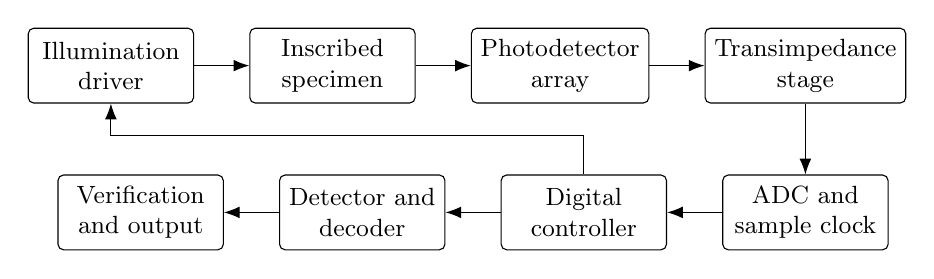
\begin{tikzpicture}[
  blk/.style={draw,rounded corners=2pt,minimum width=2.1cm,minimum height=0.95cm,align=center,font=\small},
  ar/.style={-{Latex[length=2mm]}}
]
\node[blk] (drv) {Illumination\\driver};
\node[blk,right=0.7cm of drv] (obj) {Inscribed\\specimen};
\node[blk,right=0.7cm of obj] (pd) {Photodetector\\array};
\node[blk,right=0.7cm of pd] (tia) {Transimpedance\\stage};
\node[blk,below=0.9cm of tia] (adc) {ADC and\\sample clock};
\node[blk,left=0.7cm of adc] (ctl) {Digital\\controller};
\node[blk,left=0.7cm of ctl] (dec) {Detector and\\decoder};
\node[blk,left=0.7cm of dec] (ver) {Verification\\and output};
\draw[ar] (drv)--(obj);
\draw[ar] (obj)--(pd);
\draw[ar] (pd)--(tia);
\draw[ar] (tia)--(adc);
\draw[ar] (adc)--(ctl);
\draw[ar] (ctl)--(dec);
\draw[ar] (dec)--(ver);
\draw[ar] (ctl.north) -- ++(0,0.5) -| (drv.south);
\end{tikzpicture}
\caption{Reader signal chain. The controller sequences illumination, positioning, and acquisition and passes samples to the detector and decoder; the arrow from the controller to the illumination driver represents exposure and polarization control.}
\label{fig:chain}
\end{figure}

The specification of the reader includes dynamic range, noise, sampling requirements, timing accuracy, processing throughput, power consumption, component cost, and sensitivity to misalignment. The remainder of the section derives the first two of these from the capacity model and gives a controller design for the sequencing.

\subsection{Detection noise}\label{sec:noise}

A photodiode of responsivity $\mathcal R$ illuminated by optical power $P_o$ produces a photocurrent $I=\mathcal R P_o$, which a transimpedance stage of feedback resistance $R_f$ converts to a voltage $V=-IR_f$. The current noise of such a stage at detection bandwidth $B$ has a thermal component, which is the Johnson noise of the feedback resistor,
\[
i_{\mathrm{th}}=\sqrt{\frac{4k_BTB}{R_f}},
\]
and a shot-noise component,
\[
i_{\mathrm{sh}}=\sqrt{2qIB},
\]
where $k_B$ is Boltzmann's constant, $T$ the absolute temperature, and $q$ the elementary charge. The two are independent, so their powers add. Under a standard compensated design, the closed-loop bandwidth of the stage is approximately $\sqrt{\mathrm{GBW}/(2\pi R_fC_{\mathrm{in}})}$ for an operational amplifier of gain-bandwidth product $\mathrm{GBW}$ and total input capacitance $C_{\mathrm{in}}$.

\begin{example}[Noise budget of one detection channel]\label{ex:tia}
Take $R_f=1\,\mathrm{M\Omega}$, $T=300\,\mathrm K$, $B=100\,\mathrm{kHz}$, $\mathcal R=0.5\,\mathrm{A/W}$, and $P_o=1\,\mu\mathrm W$, so that $I=0.5\,\mu\mathrm A$. The thermal noise current is $4.07\times10^{-11}\,\mathrm A$, which is $40.7$\,pA, and the shot noise current is $1.27\times10^{-10}\,\mathrm A$, which is $126.6$\,pA, so the total is $\sqrt{40.7^2+126.6^2}\approx133$\,pA. The electrical signal-to-noise ratio is $20\log_{10}\bigl(500{,}000/133\bigr)\approx71.5$\,dB. For an operational amplifier with $\mathrm{GBW}=100\,\mathrm{MHz}$ and $C_{\mathrm{in}}=10\,\mathrm{pF}$, the stage bandwidth is approximately $1.26$\,MHz, comfortably above the $100$\,kHz detection bandwidth.
\end{example}

The example shows that electronic noise in a competently designed front end is a small contribution compared with the noise sources that arise in the optics and the material, such as speckle, scattering, and specimen variation, and the program therefore characterizes the full chain empirically rather than relying on the front-end budget. Its value lies in establishing that the dynamic range needed for multilevel detection, derived next, is not limited by the electronics.

\subsection{Level resolution and the required signal-to-noise ratio}\label{sec:snr}

Suppose a single observable is used to carry one of $L$ equally spaced levels, with spacing $s$, and is read through additive Gaussian noise of standard deviation $\sigma$. A nearest-level detector places its decision thresholds at the midpoints between levels.

\begin{proposition}[Multilevel detection error and required signal-to-noise ratio]\label{prop:pam}
The symbol error probability of the nearest-level detector for $L$ equiprobable levels is
\[
P_e=2\Bigl(1-\frac1L\Bigr)Q\Bigl(\frac{s}{2\sigma}\Bigr),
\qquad Q(x)=\frac1{\sqrt{2\pi}}\int_x^\infty e^{-t^2/2}\,dt,
\]
and the average signal power of the zero-mean constellation is $s^2(L^2-1)/12$, so the signal-to-noise ratio required to achieve a given $P_e$ is
\[
\mathrm{SNR}=\frac{L^{2}-1}{12}\Bigl(\frac{s}{\sigma}\Bigr)^{2}.
\]
\end{proposition}

\begin{proof}
An interior level has two neighbours at distance $s$, and an error occurs if the noise exceeds $s/2$ in magnitude in either direction, which has probability $2Q(s/2\sigma)$. An edge level has one neighbour and error probability $Q(s/2\sigma)$. Averaging over the $L-2$ interior and $2$ edge levels gives $\bigl(2(L-2)+2\bigr)/L\cdot Q(s/2\sigma)=2(1-1/L)Q(s/2\sigma)$. For the average power, the levels are $\pm s/2,\pm 3s/2,\dots,\pm(L-1)s/2$, and the mean of their squares is $s^2(L^2-1)/12$, a standard sum. Dividing by $\sigma^2$ gives the signal-to-noise ratio.
\end{proof}

Solving for a target of $P_e=10^{-6}$ per symbol gives the requirements in Table~\ref{tab:snr}.

\begin{table}[h]
\centering
\small
\begin{tabular}{@{}rrr@{}}
\toprule
Levels $L$ & Bits per observable & Required SNR (dB) at $P_e=10^{-6}$ \\
\midrule
2 & 1 & 13.5 \\
4 & 2 & 20.7 \\
8 & 3 & 27.0 \\
16 & 4 & 33.1 \\
32 & 5 & 39.1 \\
64 & 6 & 45.1 \\
\bottomrule
\end{tabular}
\caption{Signal-to-noise ratio needed for equally spaced $L$-level detection through Gaussian noise at a symbol error probability of $10^{-6}$ before error correction.}
\label{tab:snr}
\end{table}

Each doubling of the number of levels requires about $6$\,dB of additional signal-to-noise ratio, which is the quantitative statement that bits per observable cost power linearly in decibels, and the earlier observation that halving the noise width buys one bit is the same fact in different units. For the sixteen-level case of the capacity tables the required signal-to-noise ratio is $33.1$\,dB, and the standard approximation relating the signal-to-noise ratio of an ideal converter to its resolution, $\mathrm{SNR}\approx6.02N+1.76$\,dB for an $N$-bit converter driven by a full-scale sinusoid, gives an effective resolution of about $5.2$ bits. A converter for such a channel must therefore deliver at least six effective bits after accounting for the headroom that the constellation requires, and an eight-bit converter is a conservative choice. For the twelve-property studies the converter must sustain this resolution on each of twelve observables, which can be satisfied by multiplexing one converter among the channels if the sampling rate is adequate.

\subsection{Controller design}\label{sec:controller}

The digital controller sequences the reader through alignment, calibration, scanning, decoding, and verification, and it can be specified as a finite-state machine in the standard formalism of synchronous sequential logic \cite{mano}. Let the states be IDLE, ALIGN, CALIBRATE, SCAN, DECODE, VERIFY, DONE, and FAIL, which number eight and therefore fit in three flip-flops under binary encoding or in eight under one-hot encoding. The inputs are \emph{start}, \emph{aligned}, \emph{retry}, \emph{calibrated}, \emph{scan\_done}, \emph{decoded}, \emph{more}, and \emph{enough}, where \emph{more} indicates unread blocks remain and \emph{enough} indicates that at least $k$ verified blocks have been recovered, so that the erasure code of Section~\ref{sec:ecc} can reconstruct the source. The transitions are given in Table~\ref{tab:fsm}.

\begin{table}[h]
\centering
\small
\begin{tabular}{@{}lll@{}}
\toprule
Present state & Condition & Next state \\
\midrule
IDLE & $\mathit{start}$ & ALIGN \\
ALIGN & $\mathit{aligned}$ & CALIBRATE \\
ALIGN & $\overline{\mathit{aligned}}\cdot\mathit{retry}$ & ALIGN \\
ALIGN & $\overline{\mathit{aligned}}\cdot\overline{\mathit{retry}}$ & FAIL \\
CALIBRATE & $\mathit{calibrated}$ & SCAN \\
CALIBRATE & $\overline{\mathit{calibrated}}$ & FAIL \\
SCAN & $\mathit{scan\_done}$ & DECODE \\
DECODE & $\mathit{decoded}$ & VERIFY \\
VERIFY & $\mathit{enough}$ & DONE \\
VERIFY & $\overline{\mathit{enough}}\cdot\mathit{more}$ & SCAN \\
VERIFY & $\overline{\mathit{enough}}\cdot\overline{\mathit{more}}$ & FAIL \\
\bottomrule
\end{tabular}
\caption{Controller transition table. A state not listed with a satisfied condition holds its present value, and DONE and FAIL return to IDLE on reset.}
\label{tab:fsm}
\end{table}

With one-hot encoding the next-state equations are read directly from the table. Writing each state name for the corresponding flip-flop output, the equations for three of the flip-flops are
\begin{align*}
\mathrm{ALIGN}^{+}&=\mathrm{IDLE}\cdot\mathit{start}+\mathrm{ALIGN}\cdot\overline{\mathit{aligned}}\cdot\mathit{retry},\\
\mathrm{SCAN}^{+}&=\mathrm{CALIBRATE}\cdot\mathit{calibrated}+\mathrm{SCAN}\cdot\overline{\mathit{scan\_done}}+\mathrm{VERIFY}\cdot\overline{\mathit{enough}}\cdot\mathit{more},\\
\mathrm{DONE}^{+}&=\mathrm{VERIFY}\cdot\mathit{enough}+\mathrm{DONE}\cdot\overline{\mathit{reset}},
\end{align*}
and the remaining equations follow similarly. The design is deliberately small. The controller does not decode symbols, which is the task of a separate processing block, and its function is to guarantee that a damaged specimen leads to a bounded sequence of retries rather than a hang. The \emph{enough} input embodies the central design choice that a read terminates when sufficient verified blocks have been collected and not when all blocks have been read, which lets the reader skip damaged regions at no cost.

Boylestad's analysis of linear circuits \cite{boylestad} supplies the techniques for the electrical behaviour of the front end, namely the gain, bandwidth, and noise of the amplifier stages and the response of the driver circuits, while the logic-design treatment \cite{mano} supplies the addressing, sequencing, register, and data-handling structure of the controller and its interfaces.

\subsection{Reading time and system cost}\label{sec:time}

The reading time is $T=N_{\mathrm{sites}}/(r\,n_{\mathrm{ch}})$, where $r$ is the site rate of one detection channel and $n_{\mathrm{ch}}$ the number of parallel channels. A $100$\,kHz detection bandwidth supports a site rate of order $10^{5}$ sites per second per channel, so a square metre of $10^{8}$ sites requires $10^{3}$ seconds with one channel and $100$ seconds with ten. A major design comparison concerns where complexity belongs. A carrier requiring expensive fabrication might permit a simple reader, and a cheaper inscription might demand elaborate optics and reconstruction. The research should therefore measure the complete system cost, writing and reading together, rather than optimizing inscription density alone. Writing $C_w$ for the cost of fabricating an archive of payload $S$ on a given object and $C_r$ for the cost of a reader amortized over the number $n_{\mathrm{read}}$ of times it is used, the quantity of interest is $C_w+C_r/n_{\mathrm{read}}$ at fixed $S$ and $\varepsilon$, and the optimum depends strongly on how many readings the archive is expected to receive over its life.

\section{Calibration, Discovery, and Reconstruction of the Reader}\label{sec:calibration}

Every archive includes an accessible introductory layer identifying its purpose, version, orientation, and decoding conventions, and calibration structures provide known symbols and geometric references without requiring access to the archived files. The design distinguishes aids needed for routine reading from documentation needed to reconstruct a reader from scratch. The latter must be sufficient for a competent independent party to build a functioning reader from the specimen and the specification alone, and the essential specifications are themselves redundantly distributed across the layers so that the failure of one region does not remove them.

A tiered layout serves these purposes. The outermost layer carries large features readable by eye or by an inexpensive magnifier or camera, and it states in a natural-language and pictorial form what the object is, where the denser layers are, and which standard governs them. A second layer carries medium-density structures whose decoding requires only a modest reader, and it contains the calibration symbols, the layer table, and the complete format specification in compressed text. The bulk layers carry the archive proper. This arrangement lets each tier bootstrap the next, so that an inexpensive reader can recover the specification that describes how to build a better one.

The density of calibration references is determined by how quickly the systematic offsets vary across the specimen.

\begin{proposition}[Reference density for slowly varying offsets]\label{prop:refs}
Suppose the offset field $c(x)$ is Lipschitz with constant $\lambda$ in position, so that $\|c(x)-c(x')\|\le\lambda|x-x'|$, and suppose references are placed on a square grid of spacing $g$ and each symbol is corrected by the nearest reference. The residual offset error is at most $\lambda g/\sqrt2$, and keeping it below $\eta$ requires $g\le\sqrt2\,\eta/\lambda$. With site pitch $p$, the fraction of sites devoted to references is
\[
\rho\;\ge\;\frac{p^{2}}{g^{2}}=\frac{\lambda^{2}p^{2}}{2\eta^{2}} .
\]
\end{proposition}

\begin{proof}
Every point of the plane lies within Euclidean distance $g/\sqrt2$ of some grid point, since the farthest points from a lattice node are the cell centres at distance $g/\sqrt2$. The Lipschitz condition then bounds the difference between the offset at the symbol and at its reference by $\lambda g/\sqrt2$. Requiring this to be at most $\eta$ gives the spacing condition. There is one reference per cell of area $g^2$, and the number of sites per cell is $g^2/p^2$, so the fraction of reference sites is $p^2/g^2$.
\end{proof}

The result expresses the calibration overhead in terms of measurable quantities: the rate at which the offset field varies, the tolerable residual, and the pitch. It also shows that overhead grows quadratically with the roughness of the substrate, which is one reason that rough stone and woven cloth are more demanding substrates than polished glass.

An independent-recovery experiment provides the strongest evidence of archival independence. An independent team is given a specimen and the published specification but no private calibration files or writer-side data. Successful recovery by that team gives stronger evidence of independence than repeated decoding by the team that fabricated the sample, since the latter cannot detect undocumented dependencies that its own members carry in their heads.

\section{Error Correction, Localized Damage, and Verified Recovery}\label{sec:ecc}

The archive format organizes data into independently verifiable blocks, with interleaving chosen to spread localized damage across correctable units. The relevant erasure model is natural for physical media, because scratches, missing fragments, damaged patches, and unreadable layers remove whole regions and the reader knows which regions failed when it runs a per-block integrity check.

\begin{proposition}[Block-erasure tolerance]\label{prop:mds}
An $(n,k)$ maximum-distance-separable code over a field with at least $n$ elements can reconstruct its $k$ source blocks from any $k$ surviving encoded blocks.
\end{proposition}

\begin{proof}
Take the field $\mathbb F_q$ with $q\ge n$, treat the $k$ source symbols as the coefficients of a polynomial $f$ of degree less than $k$, and define encoded symbol $j$ as $f(\alpha_j)$ for distinct field elements $\alpha_1,\dots,\alpha_n$, which is the Reed--Solomon construction \cite{reed1960}. Given any $k$ surviving encoded symbols with indices $j_1,\dots,j_k$, the linear system for the coefficients has the Vandermonde matrix $\bigl(\alpha_{j_s}^{\,t}\bigr)_{s,t}$, whose determinant is $\prod_{s<s'}(\alpha_{j_{s'}}-\alpha_{j_s})$ and is nonzero because the $\alpha$'s are distinct. The matrix is invertible, so the coefficients are uniquely determined. Applying the construction independently to each symbol position of the blocks yields the statement for blocks.
\end{proof}

\begin{proposition}[Burst tolerance by interleaving]\label{prop:burst}
Interleave the symbols of $D$ codewords, each able to correct up to $t$ symbol errors, so that consecutive transmitted symbols belong to the codewords in cyclic order. Any contiguous burst of length at most $tD$ damages at most $t$ symbols of each codeword and is therefore fully corrected.
\end{proposition}

\begin{proof}
A burst of length $\ell$ contains $\ell$ consecutive symbols, and because consecutive symbols belong to cyclically distinct codewords, each codeword receives at most $\lceil\ell/D\rceil$ of them. For $\ell\le tD$ this is at most $t$.
\end{proof}

The applications connect these familiar results to the physical failures of interest. A scratch across a surface is a burst in the scan order, and a spatial interleaver that distributes the symbols of each codeword over widely separated regions converts a scratch, a damaged corner, or a lost layer into a bounded number of erasures per codeword. The net payload of an object after calibration and coding is
\begin{equation}\label{eq:net}
B_{\mathrm{net}}=(1-\rho)\,\frac{k}{n}\,B_{\mathrm{raw}},
\end{equation}
where $\rho$ is the fraction of sites devoted to calibration and indexing and $k/n$ is the code rate. With $\rho=0.02$ and $k/n=0.8$ the net payload is $78.4\%$ of the raw payload, and this factor, a number the experiments must measure and not assume, multiplies every raw capacity quoted elsewhere in the essay.

The manuscript separates accidental-error detection from authenticity. A checksum can detect many corruptions and is inexpensive to compute. A cryptographic digest supports stronger integrity checking when the expected digest is itself trustworthy, since an attacker who can alter the object can also alter an adjacent digest. A digital signature additionally requires a trusted verification key, and the question of how that key is distributed to a reader that may have no network connection is one of the open design problems of Section~\ref{sec:stego}.

\section{Concealment, Encryption, and Public Discoverability}\label{sec:stego}

An archive meant to be publicly recoverable and an inscription meant to be unobtrusive pull in opposite directions, and the design must say, layer by layer, which property it is purchasing and at what cost. The section separates three goals that are often run together. \emph{Capacity} is the amount of information the object carries. \emph{Concealment}, in the sense of steganography, is the property that an observer who inspects the object does not learn that an inscription of a particular kind is present. \emph{Confidentiality}, in the sense of encryption, is the property that an observer who knows an inscription is present and can read it learns nothing about its content without a key. An archive of public knowledge wants capacity and discoverability, and has no use for either of the other two, while an optional protected layer might want all three. The formal separation between concealment and confidentiality rests on the observation that they are measured against different distributions, a point developed in general terms in the cryptographic literature \cite{cachin1998,hopper2002,simmons1984} and specialized here to physical inscriptions.

\subsection{Threat models}

The meaning of any security claim depends on what the observer can do. Four observers are distinguished in Table~\ref{tab:threat}. The statements of the later propositions are made relative to one of these observers, and a claim that does not name its observer is not meaningful.

\begin{table}[h]
\centering
\small
\begin{tabular}{@{}p{2.6cm}p{4.1cm}p{5.0cm}@{}}
\toprule
Observer & Capability & Relevant question \\
\midrule
Casual user & Sees and touches the object & Does the object look ordinary? \\
Inspector & Optical or electron microscopy, standard instruments & Do surface statistics differ from the substrate class? \\
Reference holder & A pristine specimen or the mold and process data & Does the object differ from the known manufacturing output? \\
Reader holder & The reader and the public specification & Can the archive be recovered, and can the protected layer be read? \\
\bottomrule
\end{tabular}
\caption{Observers against whom concealment and confidentiality claims are made.}
\label{tab:threat}
\end{table}

\subsection{Pattern repertoires are not ciphers}

An enormous pattern repertoire does not by itself establish cryptographic security, and the point can be made precisely. Suppose the mapping from patterns to symbols is public, as it must be for an open archive. Then anyone holding the object and the specification reads it, whatever the size $N$ of the repertoire, and the confidentiality is exactly zero. Suppose instead the mapping is a fixed secret bijection between a symbol alphabet of size $q$ and patterns. This is a monoalphabetic substitution, which is among the oldest ciphers and the easiest to break. Shannon's measure of how much ciphertext determines the key is the unicity distance
\begin{equation}\label{eq:unicity}
U=\frac{H(K)}{D},
\end{equation}
where $H(K)$ is the entropy of the key and $D$ is the redundancy of the plaintext in bits per symbol \cite{shannon1949}. For a secret bijection on $q=16$ symbols, $H(K)=\log_2 16!\approx 44.25$ bits, and a plaintext with redundancy $D$ bits per symbol is determined after about $44.25/D$ symbols of ciphertext, which for an uncompressed source is a few tens of symbols. Compressing the source before encoding lowers $D$ toward zero and raises $U$ correspondingly, but this only illustrates that the security would come from the key and the compression and none from the repertoire. The correct design uses a standard authenticated encryption scheme with a secret key for any protected content, and treats the pattern repertoire solely as the modulation alphabet, whose job is capacity.

\subsection{Uniform-looking inscriptions are conspicuous}

The first concealment result is the physical analogue of a basic separation between encryption and steganography. Let the natural surface texture of a substrate class, as seen by an observer, be a distribution $\mathcal T$ over $n$-site patterns, and let patterns be described by $n$ bits.

\begin{proposition}[Pseudorandom inscriptions are detectable]\label{prop:conspicuous}
Suppose there is an efficiently decidable set $S\subseteq\{0,1\}^n$ with $|S|\le2^{n/2}$ and $\Pro_{\mathcal T}[x\in S]\ge\tfrac12$, as is the case when natural textures have a correlation structure that random patterns lack. An inscription whose observed pattern is computationally indistinguishable from a uniformly random $n$-bit string is distinguished from natural texture by the observer that outputs $1$ exactly when the pattern lies in $S$, with advantage at least $\tfrac12-2^{-n/2}-\negl(n)$.
\end{proposition}

\begin{proof}
Under natural texture the observer outputs $1$ with probability at least $\tfrac12$. A uniform string lies in $S$ with probability at most $|S|/2^n\le2^{-n/2}$, and by computational indistinguishability the inscription lies in $S$ with probability at most $2^{-n/2}+\negl(n)$, since membership in $S$ is efficiently decidable and is therefore itself a distinguisher. The advantage is the difference.
\end{proof}

The consequence is that encrypting data, or compressing it to near-uniformity, before writing it makes it \emph{less} concealed on any substrate whose natural texture has structure, because ciphertext and compressed data look random and natural textures do not. A strongly secret inscription is not a hidden one, and the two goals must be pursued by different mechanisms.

\subsection{How much can be hidden}

Two bounds characterize concealed capacity, according to whether the observer uses the same instrument as the reader or a coarser one. Write $R$ for the reader's observation of a site, $W$ for the observer's observation, and suppose the observer's observation is a function $W=\phi(R)$ of the reader's, so that the observer sees no more than the reader.

\begin{proposition}[Concealed capacity with a coarser observer]\label{prop:fiber}
Consider a keyed inscription of $n$ sites carrying a uniformly random payload $M$ of $B$ bits, recovered exactly from the reader's observations $R^{n}$ and the key $K$, and perfectly concealed in the sense that the observer's pattern $W^{n}$ has its natural distribution whatever $M$ is. Let $N_w=|\phi^{-1}(w)|$ be the number of reader-distinguishable states compatible with the observation $w$. Then
\[
B\le\max_{w^{n}}\sum_{i=1}^{n}\log_2 N_{w_i}.
\]
If in addition the natural distribution of $R$ is uniform on each fibre $\phi^{-1}(w)$, the bound is achieved with equality when each $N_w$ is a power of two.
\end{proposition}

\begin{proof}
Because the payload is recovered exactly, $H(M\mid R^{n},K)=0$, and since $M$ is independent of $K$ we have $B=H(M)=H(M\mid K)=I(M;R^{n}\mid K)$. As $W^{n}$ is a function of $R^{n}$, the chain rule gives $I(M;R^{n}\mid K)=I(M;W^{n}\mid K)+I(M;R^{n}\mid W^{n},K)$. The first term is zero because $W^{n}$ has the same distribution for every value of $M$ and $K$, so it is independent of both. The second is at most $H(R^{n}\mid W^{n})$, which is at most the logarithm of the number of $R^{n}$ compatible with $W^{n}$, namely $\sum_i\log_2N_{w_i}$, maximized over $w^n$. For achievability, if the natural distribution is uniform on each fibre, choose the reader state within the fibre of the natural observation $w_i$ according to $\log_2N_{w_i}$ bits of the (uniform) payload; the resulting joint distribution of $(R,W)$ is exactly the natural one, and the reader, who can compute $W=\phi(R)$ and hence the fibre, recovers the bits from the index within the fibre.
\end{proof}

The bound has a clean reading. Concealed capacity is the logarithm of the number of reader-distinguishable states that hide behind each observation the warden can make, and it is the quantity that multidimensional encodings enlarge. A site observed by an inspector only through its optical transmission intensity, but by the reader through retardance and slow-axis orientation as well, has a large fibre, and an inscription written entirely in the hidden dimensions leaves the inspector's observation unchanged. This is the formal content of the intuition that laser-written structures in glass can be nearly invisible to the eye and still carry data.

When the observer uses the same instrument as the reader, the fibre has one element and the proposition gives zero, which is the case where the information-theoretic entropy bound applies.

\begin{proposition}[Concealed capacity with an identical observer]\label{prop:entropy}
Let the natural pattern of $n$ sites be i.i.d.\ with per-site distribution $P$ of entropy $H(P)$. If a keyed inscription carrying a uniformly random payload of $B$ bits is perfectly concealed, meaning that the observed pattern is distributed exactly as $P^{n}$, and the payload is recovered exactly from the pattern and the key, then $B\le nH(P)$.
\end{proposition}

\begin{proof}
Let $Y^{n}$ be the observed pattern. Exact recovery gives $H(M\mid Y^{n},K)=0$, so $B=H(M)=H(M\mid K)=I(M;Y^{n}\mid K)\le H(Y^{n}\mid K)\le H(Y^{n})=nH(P)$, where the last equality uses the perfect concealment assumption.
\end{proof}

The bound is achieved asymptotically by distribution matching, in which the payload bits, followed by fresh random bits, drive an arithmetic decoder for the natural distribution, so that the output has the natural law while the payload is recoverable by an arithmetic encoder \cite{cover2006}. The proposition says that if the instrument can see everything the reader sees, concealed capacity is limited by the natural entropy of the substrate, and is zero for a perfectly deterministic process. Table~\ref{tab:hidden} shows the scale for a surface of $10^{8}$ sites per square metre.

\begin{table}[h]
\centering
\small
\begin{tabular}{@{}rr@{}}
\toprule
Natural entropy $h$ per site (bits) & Concealed capacity per square metre \\
\midrule
0.5 & 6.25\,MB \\
2 & 25\,MB \\
8 & 100\,MB \\
\bottomrule
\end{tabular}
\caption{Concealed capacity per square metre under Proposition~\ref{prop:entropy} for an identical observer, at $10^{8}$ sites per square metre, as a function of the natural entropy of the substrate per site.}
\label{tab:hidden}
\end{table}

For comparison, the ideal overt capacity of the twelve-property case is $0.6$\,GB per square metre, so identical-observer concealment costs one to two orders of magnitude of capacity unless the substrate is highly variable. A consequence that bears on manufacturing is that mass-produced identical units are a poor cover against an observer who holds a reference specimen, since the natural entropy is only the process variability, whereas handmade or naturally heterogeneous substrates such as fired clay and quarried stone have much more.

\subsection{Composition and the dual-layer design}

The two goals compose in one order, as in the general setting.

\begin{proposition}[Encrypt, then embed]\label{prop:compose}
Let $\mathsf{Enc}_{k_1}$ produce pseudorandom ciphertexts under chosen-plaintext attack and let the embedding be concealed for uniformly random payloads under key $k_2$. The embedding of $\mathsf{Enc}_{k_1}(m)$ under $k_2$ is concealed, and an observer who learns $k_2$ still faces the chosen-plaintext security of $\mathsf{Enc}_{k_1}$.
\end{proposition}

\begin{proof}
Replace $\mathsf{Enc}_{k_1}(m)$ by a uniform string of the same length; the change is undetectable by the pseudorandomness of ciphertexts. The embedding of a uniform payload is, by assumption, indistinguishable from natural texture. An observer who learns $k_2$ and extracts the embedded string obtains $\mathsf{Enc}_{k_1}(m)$ only.
\end{proof}

By Proposition~\ref{prop:conspicuous} the reverse order, embedding and then encrypting, yields a pseudorandom pattern that is conspicuous. The proposition therefore says that encryption serves concealment as a preprocessing step that supplies uniform payload bits and does not provide concealment itself.

The architectural consequence is a dual-layer design in which an accessible public reference archive coexists with optional protected data. The public layer is overt, carries the introductory inscription, and uses an open decoding method, so its capacity is limited by the engineering of Sections~\ref{sec:capacity} through~\ref{sec:ecc} and not by concealment. The protected layer is written in dimensions the casual and inspector observers do not see, as in Proposition~\ref{prop:fiber}, encrypted under a key held outside the object, and accounted for separately, so that the total payload is $B_{\mathrm{pub}}+B_{\mathrm{prot}}$ and the loss of the key destroys only $B_{\mathrm{prot}}$. The design contains an honest tension. The presence of an obvious public archive raises the prior that the object carries more than it shows, and an object that proclaims itself an archive is a worse cover than one that does not, so a deployment must decide whether the protected layer is to be concealed or merely confidential. An authentic archive also needs a verification key distributed to readers who may be offline, and the principle of replication proposed for the archives applies to the key fingerprint as well: publishing the fingerprint in many places, including the introductory layers of many objects, lets a reader cross-check a signature against several independent sources.

\section{The Experimental Sequence: Twelve, One Hundred Forty-Four, and Thirteen Thousand Parameters}\label{sec:experiments}

The twelve-parameter study establishes a fully inspectable baseline. Candidate controls are varied individually and jointly to measure coupling, repeatability, and incremental information gain, and the study does not require all twelve to survive screening. A screening statistic is needed that attributes recoverable information to each control without requiring the full joint codebook to be written.

\begin{proposition}[Marginal information lower-bounds joint information]\label{prop:marg}
Let the fabrication controls $U_1,\dots,U_d$ be independent random variables, and let $Y$ be the observation. Then
\[
I(U_1,\dots,U_d;Y)\;\ge\;\sum_{i=1}^{d}I(U_i;Y).
\]
\end{proposition}

\begin{proof}
By the chain rule, $I(U_1,\dots,U_d;Y)=\sum_iI(U_i;Y\mid U_1,\dots,U_{i-1})$. For each $i$, independence of the controls gives $I(U_i;U_1,\dots,U_{i-1})=0$, so $I(U_i;Y\mid U_{<i})=I(U_i;Y,U_{<i})-I(U_i;U_{<i})=I(U_i;Y,U_{<i})\ge I(U_i;Y)$, using that adding variables to the second argument cannot decrease mutual information. Summing over $i$ gives the claim.
\end{proof}

The proposition makes one-at-a-time screening informative: if each control is varied independently and its marginal mutual information with the observation is estimated from a measured confusion matrix, the sum of the estimates is a lower bound on the information carried by the full joint codebook when the controls are written independently. The bound can be loose, since interactions can add information, but it never overstates the achievable payload, which is the safe direction for a research program that wishes to avoid inflated claims. The effective alphabet size of a control can then be reported as $2^{\hat I_i}$ with $\hat I_i$ the estimate.

The one-hundred-forty-four-parameter study investigates structured arrays, repeated mode families, and hierarchical readout. It compares physically adding independent observables with merely adding more adjustable coefficients to a model, in the sense of Section~\ref{sec:fixed}. The thirteen-thousand-parameter study begins computationally, using a declared forward model and realistic resource constraints. A fabricated specimen follows only if simulation and the smaller experiments support identifiable, robust modes, and throughout the study ``13,000 parameters'' remains a description of the model or control space until recoverable information has been measured. Table~\ref{tab:stages} summarizes the sequence.

\begin{table}[h]
\centering
\small
\begin{tabular}{@{}p{2.1cm}p{3.8cm}p{3.9cm}p{2.3cm}@{}}
\toprule
Stage & Activity & Decision statistic & Proceed if \\
\midrule
$d=12$ & Fabricate coupons; vary controls singly and jointly; read with the baseline reader & Marginal $\hat I_i$ per control; confusion matrices; $\sigma_{\min}$ of the mixing matrix & Total $\sum_i\hat I_i$ exceeds binary baseline net of overhead \\
$d=144$ & Structured arrays and hierarchical readout on the best substrate & Net payload per area at stated $\varepsilon$; singular-value spectra & Net density exceeds $d=12$ at equal cost \\
$d=13{,}000$ & Simulation with declared forward model; specimen only if supported & Identifiable rank; capacity under fixed power (Prop.~\ref{prop:gauss}) & Rank and SNR survive resource constraints \\
\bottomrule
\end{tabular}
\caption{Staged experimental sequence and the decision statistic that governs progression.}
\label{tab:stages}
\end{table}

For every scale, the decisive output is the net recovered payload per area or volume, at a specified error rate, reading time, writing time, and cost.

A statistical rule governs the reporting of error rates. To claim that a block error probability does not exceed $\varepsilon$ with confidence $1-\alpha$ from trials that produced no failures, the number of independent trials must satisfy $(1-\varepsilon)^{N}\le\alpha$, which is the probability of observing no failures if the true error rate were $\varepsilon$, and therefore
\[
N\ge\frac{\ln(1/\alpha)}{-\ln(1-\varepsilon)}\approx\frac{\ln(1/\alpha)}{\varepsilon}.
\]
For $\alpha=0.05$ this is approximately $3/\varepsilon$, so establishing a block error rate below $10^{-3}$ at ninety-five percent confidence requires about three thousand failure-free trials, and the experimental design must budget for that scale of repetition.

\section{Baselines, Controls, and Falsification}\label{sec:controls}

The proposal compares its candidates with simpler patterns fabricated using the same equipment, substrate, area, and time budget. The principal baseline is a binary encoding, one bit per site, which is the format of most existing optical media, together with a multilevel encoding of a single observable. A complicated optical encoding should earn its complexity by improving a declared metric, namely net recovered payload per unit area at fixed error rate and cost, and the comparison must be run on specimens fabricated in the same batch to remove the confounding effect of process drift.

Experiments use previously unseen payloads and report unsuccessful reads. Recovering random payloads establishes storage without relying on source redundancy, and recovering compressed documents demonstrates an archival workflow. Decoder training data and dictionaries are disclosed and included in the accounting, in accordance with the side-information correction of Section~\ref{sec:overlap}, whenever they contain source-specific information. Reports include the full distribution of block outcomes, including failures, rather than only the best specimens.

The program explicitly permits negative results. Added controls might provide no independent information, which Proposition~\ref{prop:equiv} identifies as the expected outcome for controls that merely change the fabrication recipe. Fabrication variation might overwhelm multilevel encoding, so that the usable number of levels is small and the payload falls toward the binary baseline. Calibration overhead might eliminate a raw-density advantage, as in Proposition~\ref{prop:refs}. Reader cost might exceed the benefit of density. Each such outcome would still identify useful limits and guide better designs, and the program is organized so that these are measured and reported and not discovered after the fact.

\section{Distributed Archives and Correlated Survival}\label{sec:distribution}

At the architectural level the paper distinguishes unique stored content from replicated content, and replication is the second source of value identified in Section~\ref{sec:intro}.

\begin{proposition}[Conditional replication benefit]\label{prop:repl}
If $r$ complete copies fail independently with probability $p$ each, the probability that all copies fail is $p^{r}$.
\end{proposition}

\begin{proof}
The event that all fail is the intersection of the independent failure events, whose probability is the product $p^{r}$.
\end{proof}

The next paragraph examines the assumption. Copies can share a vulnerable reader, a material, a decoder, a manufacturing defect, or an institution, and these are common-mode failures.

\begin{proposition}[Common-mode floor]\label{prop:common}
Suppose a common-mode event destroys access to all copies with probability $q$, independently of the copies' individual failures, and each of $r$ copies otherwise fails independently with probability $p$. The probability that the archive is lost is
\[
q+(1-q)\,p^{r}\;\ge\;q ,
\]
which cannot be reduced below $q$ by adding copies.
\end{proposition}

\begin{proof}
The archive is lost if the common-mode event occurs, which has probability $q$, or if it does not occur, with probability $1-q$, and all $r$ copies fail independently, with probability $p^r$. The two cases are disjoint and the sum gives the formula. Since $(1-q)p^{r}\ge0$, the loss probability is at least $q$.
\end{proof}

With $p=0.1$ and $q=10^{-3}$, the loss probability is $0.1009$ for one copy, $0.0110$ for two, $0.0020$ for three, $0.0011$ for four, and $0.001001$ for six, so beyond about four copies further replication buys almost nothing, because the common-mode term dominates. The research program therefore studies diversity of substrate, geography, reader implementation, and documentation as the means of reducing $q$, which is the variable that replication itself cannot address. A million inscriptions that depend on a single unavailable decoding service have extensive physical replication but limited operational independence.

A collection must also be defined as a bounded object. A dated encyclopedic release, a technical reference library, and a collection of scientific articles can be measured and verified, whereas ``the internet'' is a popular shorthand for many selected collections that change and cannot be preserved as a single readable snapshot. Immutable releases carry manifests, content identifiers, provenance, and explicit dates. Updates can be distributed as complete new copies or as deltas, and the latter create dependencies on earlier versions.

\begin{proposition}[Cost of delta chains]\label{prop:delta}
Suppose each version is held by $m$ independent copies, each surviving with probability $s$, so that version availability is $a=1-(1-s)^{m}$. If recovering version $v$ requires all of the $v$ versions in its chain, and versions are independent, the availability of version $v$ is $a^{v}$, whereas a complete snapshot of version $v$ has availability $a$.
\end{proposition}

\begin{proof}
The chain is available only if every one of its $v$ links is, and the links are independent, so the probability is the product $a^{v}$. A snapshot depends on a single link.
\end{proof}

For $a=0.99$, a chain of twenty versions has availability $0.99^{20}\approx0.82$ and a chain of one hundred versions has $0.99^{100}\approx0.37$. The design problem therefore concerns how much historical independence to preserve: a slightly larger complete snapshot might be more useful after institutional disruption than a smaller update that requires several missing predecessors, and periodic complete snapshots bound the length of every chain.

\section{The Library in the Environment}\label{sec:popular}

The preceding sections were deliberately austere, and this one returns to the central images of the program in a less formal register while keeping the arithmetic honest. The images are walls carrying reference collections, furniture carrying repair libraries, garments transporting small archives, and inexpensive objects dispersing public knowledge through ordinary circulation. The question that makes them more than whimsy is quantitative: how much surface does a useful archive need?

Using the net factor of $0.784$ from equation~\eqref{eq:net} and the ideal raw densities of Table~\ref{tab:area}, Table~\ref{tab:area-needed} gives the area required to carry an archive of illustrative size $S$. The sizes of one and one hundred gigabytes are chosen to span the scale of a substantial text collection and of a much larger multimedia collection, and they are not claims about the size of any particular collection.

\begin{table}[h]
\centering
\small
\begin{tabular}{@{}rrr@{}}
\toprule
Properties per site & Area for $S=1$\,GB & Area for $S=100$\,GB \\
\midrule
12 & $2.13\ \mathrm{m^2}$ & $213\ \mathrm{m^2}$ \\
144 & $0.177\ \mathrm{m^2}$ & $17.7\ \mathrm{m^2}$ \\
13{,}000 & $19.6\ \mathrm{cm^2}$ & $0.196\ \mathrm{m^2}$ \\
\bottomrule
\end{tabular}
\caption{Surface area needed to carry an archive of size $S$ at $100\,\mu\mathrm m$ pitch, sixteen levels per property, and net factor $0.784$. All figures are conditional on the idealizations of the preceding sections.}
\label{tab:area-needed}
\end{table}

The difference between the rows is the difference between an archive spread across a building and an archive that fits on a small tile. A standard brick has a stretcher face of about $215\times65$\,mm, which is roughly $0.014\ \mathrm{m^2}$, and at the same assumptions its face carries a net payload of about $6.6$\,MB in the twelve-property case, $79$\,MB in the one-hundred-forty-four-property case, and $7.1$\,GB in the thirteen-thousand-property case. The first of these is a library of reference text, the second a substantial technical corpus, and the third a large collection. None is measured, and each is a target that the experimental sequence of Section~\ref{sec:experiments} is designed to confirm or refute.

Two deliberately absurd scenarios illustrate the proposition behind the program in an exaggerated form, and their value is that they make a structural point vivid. The first is the crumpled paper ball, a sheet carrying an archive that is folded into a compact object so that a negligible-looking thing contains an unexpectedly consequential collection. Crumpling does not itself compress the information, because folding changes the geometry and accessibility of the carrier and leaves the encoded representation unchanged, and any reduction in the length of the encoded representation requires a separate compression method acting on the source. The distinction is productive: it separates the physical smallness of an object, which depends on how the carrier occupies space, from the informational smallness of its content, which depends on redundancy in the source, and the program's mathematics concerns only the second and the density of the carrier. A culture's knowledge becomes materially small without becoming informationally trivial.

The second is an edible or biodegradable carrier, given the deliberately provocative label ``weaponized manna'' for a speculative distribution scenario in which a perishable object carries a durable collection. The tension is that ordinary use of each individual carrier destroys its inscription, and the question becomes whether the archive as a whole persists when its carriers are consumed. A simple model captures the answer. Let each copy independently be lost at rate $\mu$ and independently produce a new copy at rate $\beta$, so that the number of copies is a linear birth--death process.

\begin{proposition}[Persistence of perishable copies]\label{prop:birthdeath}
Starting from one copy, the probability that the archive eventually becomes extinct is $\min(1,\mu/\beta)$, and starting from $N_0$ independent copies it is $\min(1,\mu/\beta)^{N_0}$. In particular, the archive persists with positive probability if and only if the copying rate exceeds the loss rate.
\end{proposition}

\begin{proof}
Condition on the first event experienced by a single copy. With probability $\mu/(\beta+\mu)$ it is a loss, and the lineage is extinct. With probability $\beta/(\beta+\mu)$ it is a birth, after which there are two independent copies, each of whose lineages goes extinct with the same probability $q$. Hence $q=\dfrac{\mu}{\beta+\mu}+\dfrac{\beta}{\beta+\mu}\,q^{2}$, which rearranges to $\beta q^{2}-(\beta+\mu)q+\mu=0$, and factoring gives $(q-1)(\beta q-\mu)=0$. The extinction probability is the smallest nonnegative root, which is $\mu/\beta$ if $\mu<\beta$ and $1$ otherwise. Independent lineages multiply, which gives the second statement.
\end{proof}

The proposition formalizes the earlier remark that an edible carrier introduces a tension between individual perishability and collective persistence: each individual copy is expendable, and the archive survives if reproduction of copies, which is a social and manufacturing process, outpaces their consumption. Whether such a carrier is feasible is a separate materials question, including whether the inscription survives handling and whether the carrier remains suitable for its intended use, and nothing in the argument depends on its answer.

The decisive requirement across all of these scenarios is recoverability without the institution that produced the object. A wall containing a magnificent archive would offer limited independence if reading it required a proprietary scanner, a cloud account, or an undocumented decoding model. A stronger design, as Section~\ref{sec:calibration} specified, carries a readily recognizable introductory inscription that explains the format, the calibration marks, the error correction, and the reader requirements, with progressively denser layers holding the larger collection, so that the object preserves enough instructions to help reconstruct its own means of access. The larger possibility is that archival replication becomes an ordinary consequence of making things. A brick could carry a library alongside its maker's mark, and a table could arrive with reference works embedded beneath its finish. Even modest capacity, repeated across enough ordinary objects with an open reading method, could produce substantial independence from centralized storage, and its value depends on whether people can recognize, read, verify, and maintain those archives across generations.

\section{Publication Program and Open Problems}\label{sec:program}

The program yields a coherent sequence of papers. A theoretical article would treat distinguishable material states and capacity bounds, comprising the results of Sections~\ref{sec:capacity} through~\ref{sec:fixed}. An experimental article would address a specific substrate, with the staged measurements of Section~\ref{sec:experiments}. A circuits article would address the reader, comprising Section~\ref{sec:reader} and the calibration and error-correction material, and it is the natural contribution for a circuits and design venue. A systems article would address distributed archival manufacture, comprising Sections~\ref{sec:distribution} and~\ref{sec:popular}. The long foundational essay explains how these contributions fit together without presenting projected experiments as completed achievements.

Several problems are explicitly open. The first is empirical and central: for each substrate, the function $b(p)$ of Section~\ref{sec:geometry} that relates payload per site to site pitch has not been measured, and the viability of the program depends on its shape. The second is the effective rank of the mixing matrix of Section~\ref{sec:linear} for large numbers of nominally independent optical properties, where the proof techniques here give only sufficient conditions. The third is concealment against an observer who uses the same instrument as the reader on a substrate with little natural entropy, where Proposition~\ref{prop:entropy} says that very little can be hidden and no construction here improves on that. The fourth is the offline distribution of trust, that is, how a reader with no network connection obtains a verification key it can believe, for which the replication of key fingerprints across many objects is proposed here and has not been analyzed. The fifth is standardization: the introductory layer, the container format of Appendix~\ref{app:format}, and the calibration conventions must be stable enough for independent teams to build compatible readers, and the experience of other archival formats suggests that this is as much a social as a technical problem.

The central thesis can now be stated in the form that the analysis supports. Multidimensional optical encoding may make ordinary manufactured objects useful carriers of substantial public archives, but its capacity must be established through independently recoverable information, and its archival value through independently sustainable access. The astronomical combinatorics of the address space, the overlapping inscriptions, and the radical distribution of copies are all part of the picture, and each enters the argument in its proper place: the first as an address space, the second as a constraint on joint distinguishability, and the third as a sociotechnical multiplier whose effect is limited by common-mode failures.

\appendix

\section{Notation}\label{app:notation}

\begin{table}[h]
\centering
\small
\begin{tabular}{@{}ll@{}}
\toprule
Symbol & Meaning \\
\midrule
$d$ & Number of independent properties or modes per site \\
$L_i$ & Number of reliably distinguishable levels of property $i$ \\
$M$, $b$ & Number of joint states; payload bits per site, $b=\lfloor\log_2M\rfloor$ \\
$p$, $A$, $V$ & Site pitch; usable area; usable volume \\
$B_{\mathrm{raw}}$, $B_{\mathrm{net}}$ & Raw and net payload of an object \\
$\rho$, $k/n$ & Calibration fraction; code rate \\
$H$, $\sigma_{\min}$ & Mixing matrix; its smallest singular value \\
$\delta$, $\varepsilon$ & Readout noise bound; target error probability \\
$R_f$, $B$ & Feedback resistance; detection bandwidth \\
$s$, $\sigma$ & Level spacing; noise standard deviation \\
$p$, $q$, $r$ & Copy failure probability; common-mode probability; number of copies (context decides) \\
\bottomrule
\end{tabular}
\end{table}

\section{Worked Budget for a One-Square-Centimetre Coupon}\label{app:budget}

A coupon of area $1\ \mathrm{cm^2}$ at $100\,\mu\mathrm m$ pitch has $10^{4}$ sites. The raw payload and the net payload, using the factor $0.784$ from equation~\eqref{eq:net}, are given in Table~\ref{tab:coupon} for the three parameter counts of the essay with sixteen levels per property.

\begin{table}[h]
\centering
\small
\begin{tabular}{@{}rrrr@{}}
\toprule
Properties per site & Bits per site & Raw payload & Net payload \\
\midrule
12 & 48 & 60\,kB & 47.0\,kB \\
144 & 576 & 720\,kB & 564\,kB \\
13{,}000 & 52{,}000 & 65\,MB & 51.0\,MB \\
\bottomrule
\end{tabular}
\caption{Coupon budget: $10^{4}$ sites, decimal units, $\rho=0.02$ and $k/n=0.8$.}
\label{tab:coupon}
\end{table}

The coupon is the natural unit of the first experiments. A coupon of the first row is large enough to hold a complete specification document together with a test file of tens of kilobytes, and it can be written and read in minutes with the reader of Section~\ref{sec:reader}, which makes the twelve-parameter study feasible at small scale.

\section{A Container Format for the Introductory and Archive Layers}\label{app:format}

The following grammar is a sketch of the container that Section~\ref{sec:calibration} requires, intended to be implementable by an independent party from the text of the specification alone.
\begin{verbatim}
Archive   := Sentinel Intro Calib LayerTable Manifest Block*
Sentinel  := fixed pattern, rotation-invariant, repeated at corners
Intro     := plain-language statement, version, pointer to LayerTable
Calib     := reference symbols for every observable, on a grid
             of spacing g (Prop. refs), known nominal values
LayerTable:= (layer id, depth, pitch, observables, levels) per layer
Manifest  := (block id, digest, size, role) per block, signed
Block     := Header Payload Digest
Header    := block id, layer id, code (n, k), stripe index
Payload   := coded symbols, spatially interleaved (Prop. burst)
Digest    := cryptographic hash of Payload before coding
\end{verbatim}
The manifest lists every block with its digest so that a reader can verify each recovered block independently and stop as soon as the \emph{enough} condition of Table~\ref{tab:fsm} holds.

\section{Estimating Information from Confusion Matrices}\label{app:estimate}

The screening of Section~\ref{sec:experiments} requires estimates of mutual information from finite measurements. Given $N$ labelled trials of a control with $|X|$ settings and an observation quantized into $|Y|$ bins, the plug-in estimate of $I(X;Y)$ from the empirical joint frequencies is biased upward by approximately
\[
\frac{(|X|-1)(|Y|-1)}{2N\ln2}\ \text{bits}
\]
for large $N$ \cite{miller1955}, and the bias must be subtracted or the experiments made large enough that it is negligible. Intervals for the block error rate follow from the rule of Section~\ref{sec:experiments}, and the program reports the estimates with their uncertainties, never as point values alone.

\begin{thebibliography}{99}
\bibitem{anderson2023} P. Anderson et al. Project Silica: Towards sustainable cloud archival storage in glass. \emph{Proceedings of the 29th ACM Symposium on Operating Systems Principles (SOSP)}, 166--181, 2023.
\bibitem{boylestad} R. L. Boylestad, D. Edgar, J. Jenness, J. Tompkin. \emph{Boylestad's Circuit Analysis}, second Canadian edition.
\bibitem{cachin1998} C. Cachin. An information-theoretic model for steganography. \emph{Information Hiding}, 1998.
\bibitem{cheriere2025} N. Cheriere et al. Holographic storage for the cloud: advances and challenges. \emph{ACM Transactions on Storage} 21(1), article 3, 2025.
\bibitem{coufal2000} H. J. Coufal, D. Psaltis, G. T. Sincerbox, editors. \emph{Holographic Data Storage}. Springer Series in Optical Sciences 76. Springer, 2000.
\bibitem{cover2006} T. M. Cover, J. A. Thomas. \emph{Elements of Information Theory}, second edition. Wiley, 2006.
\bibitem{epp} S. S. Epp. \emph{Discrete Mathematics with Applications}, fourth edition.
\bibitem{fan2024} Z. Fan et al. Holographic multiplexing metasurface with twisted diffractive neural network. \emph{Nature Communications} 15, 9416, 2024.
\bibitem{hopper2002} N. Hopper, J. Langford, L. von Ahn. Provably secure steganography. \emph{CRYPTO}, 2002.
\bibitem{kolman} B. Kolman, R. C. Busby, S. C. Ross. \emph{Discrete Mathematical Structures}, fifth edition.
\bibitem{mano} M. M. Mano, C. R. Kime. \emph{Logic and Computer Design Fundamentals}, third edition.
\bibitem{miller1955} G. A. Miller. Note on the bias of information estimates. In H. Quastler, editor, \emph{Information Theory in Psychology}, 1955.
\bibitem{reed1960} I. S. Reed, G. Solomon. Polynomial codes over certain finite fields. \emph{Journal of the Society for Industrial and Applied Mathematics} 8(2), 300--304, 1960.
\bibitem{ren2020} H. Ren, X. Fang, J. Jang, J. B\"urger, J. Rho, S. A. Maier. Complex-amplitude metasurface-based orbital angular momentum holography in momentum space. \emph{Nature Nanotechnology} 15, 948--955, 2020.
\bibitem{shannon1948} C. E. Shannon. A mathematical theory of communication. \emph{Bell System Technical Journal} 27, 379--423 and 623--656, 1948.
\bibitem{shannon1949} C. E. Shannon. Communication theory of secrecy systems. \emph{Bell System Technical Journal} 28, 656--715, 1949.
\bibitem{silica2026} Microsoft Research Project Silica Team. Laser writing in glass for dense, fast and efficient archival data storage. \emph{Nature} 650, 606--612, 2026.
\bibitem{simmons1984} G. J. Simmons. The prisoners' problem and the subliminal channel. \emph{CRYPTO}, 1983 (published 1984).
\bibitem{wang2022} H. Wang et al. 100-layer error-free 5D optical data storage by ultrafast laser nanostructuring in glass. \emph{Laser \& Photonics Reviews} 16(4), 2100563, 2022.
\bibitem{zhang2013} J. Zhang, M. Gecevi\v{c}ius, M. Beresna, P. G. Kazansky. 5D data storage by ultrafast laser nanostructuring in glass. \emph{CLEO: 2013 Postdeadline Paper Digest}, paper CTh5D.9. Optical Society of America, 2013.
\end{thebibliography}


\end{document}
